\section{Rates as halo functionals}\label{sec:21.1}

The silicon rate of \cref{sec:10.2-corrections}, \num{5.9e4} events per kilogram and year at \SI{10}{MeV} for $\sigmae = \SI{e-37}{cm^2}$ with the random-phase loss function with local fields, rests on one velocity distribution, the standard halo of \cref{sec:1.2}. Simulated galaxies hold dark matter that this distribution does not describe. In the Via Lactea~II simulation, for instance, 22 percent of the dark matter near the Sun's radius is debris stripped from satellites that still survive, and it moves at a galactic speed near \SI{340}{km.s^{-1}}~\cite{kuhlen2012direct}. A limit compared with such a halo has to be recomputed, and the recomputation is cheap because every rate in this book is linear in $f_\chi$. We will write the rate of any channel as one integral of $f_\chi$ against a kernel that holds everything else: the coupling, the response, the kinematics and the readout.

\subsection{The halo functional of a channel}\label{sec:21.1-functional}

A detector counts events in bins of some observable, the number of pairs $N_{\mathrm{eh}}$ for a charge readout. The rate in one bin is \cref{eq:8.7-handoff}. In it the velocity integral is the outermost one, and everything inside it depends on $\vect{v}$ but not on the halo. We collect it into one function:
\begin{keyresult}[Halo functional of a channel]
\begin{equation}
  \mathcal{R}_{N_{\mathrm{eh}}}[f_\chi] = \frac{\rho_\chi}{\mchi\,\rho_T}\int\dd^3v\,f_\chi(\vect{v})\,\varGamma_{N_{\mathrm{eh}}}(\vect{v}) ,
  \label{eq:21.1-functional}
\end{equation}
with the \emph{rate kernel}, the inner integrals of \cref{eq:8.7-handoff} at fixed $\vect{v}$,
\begin{equation}
  \varGamma_{N_{\mathrm{eh}}}(\vect{v}) = \int\frac{\dd^3q}{(2\pi)^3}\sum_\Lambda\sum_{a,b}\mathfrak{D}_{ab}(\vect{q},\vect{v})\,S_{ab}(\vect{q},\omega_{\vect{q}};\Lambda)\,P_{\mathrm{casc}}(N_{\mathrm{eh}}|\Lambda) ,
  \label{eq:21.1-kernel}
\end{equation}
the rate at which one dark-matter particle of velocity $\vect{v}$ makes events with $N_{\mathrm{eh}}$ pairs.
\end{keyresult}
\noindent Summed over $N_{\mathrm{eh}}$, the kernel is the per-particle rate $\varGamma(\vect{v})$ of \cref{eq:8.2-rate}. For any other observable, a phonon energy or a bin of total deposited energy, $P_{\mathrm{casc}}$ is replaced by the probability that the event lands in that bin. The halo enters only through $f_\chi$ and $\rho_\chi$, the channel only through its kernel, and the rate is a linear functional of $f_\chi$: a halo made of two components gives the sum of their rates, weighted by their shares of the density.

The kernel is never negative, since $\mathfrak{D}$ and $S$ are positive semidefinite matrices (\cref{sec:8.2}) and $P_{\mathrm{casc}}$ is a probability. Adding dark matter at any velocity therefore never lowers a rate, which is the property on which the halo-independent bounds of \cref{sec:21.2} rest. The kernel vanishes at small speeds. A particle of speed $v$ reaches only the pairs $(q,\omega)$ with $\vmin(q,\omega) \le v$ (\cref{sec:1.3}), so $\varGamma(\vect{v}) = 0$ for $v$ below the onset speed $v_{\mathrm{on}}(\mchi)$, the smallest $\vmin$ over the support of the response. And for a crystal the kernel depends on the direction of $\vect{v}$ in crystal axes. The laboratory distribution is $f_{\mathrm{gal}}(\vect{v} + \vect{v}_{\mathrm{E}}(t))$ (\cref{eq:1.2-flab}), and the crystal turns with the Earth (\cref{eq:1.2-rotation}). Averaged over an exposure, \cref{eq:21.1-functional} becomes
\begin{equation}
  \bar{\mathcal{R}}_{N_{\mathrm{eh}}} = \frac{\rho_\chi}{\mchi\,\rho_T}\int\dd^3v_{\mathrm{gal}}\,f_{\mathrm{gal}}(\vect{v}_{\mathrm{gal}})\,\bigl\langle\varGamma_{N_{\mathrm{eh}}}\bigl(\vect{v}_{\mathrm{gal}} - \vect{v}_{\mathrm{E}}(t)\bigr)\bigr\rangle_t ,
  \label{eq:21.1-exposure}
\end{equation}
where $\langle\cdot\rangle_t$ averages over the live time, with the argument of $\varGamma$ rotated into crystal axes at each $t$. All time dependence is now in the kernel, and the exposure-averaged kernel at $\vect{v}_{\mathrm{gal}}$ is the rate that a single stream of dark matter at that velocity would produce.

Absorption fits the same form. The kernel is then $\varGamma_{\mathrm{abs}}$ of \cref{eq:8.2-abs}, which depends on $\vect{v}$ only through the momentum $\vect{p}_\phi = m_\phi\vect{v}$ and the energy $\omega_\phi \simeq m_\phi(1 + v^2/2)$. Where the response is smooth on the scale $m_\phi v \approx 10^{-3}m_\phi$, the kernel is constant across the halo and the rate depends on the halo through $\rho_\chi$ alone.

\subsection{The mean inverse speed}\label{sec:21.1-eta}

For a response averaged over the directions of $\vect{q}$, as in the crystal form factor of \cref{sec:10.1}, the kernel depends only on the speed. The angular average of the energy delta function is $\Theta(v - \vmin)/(2qv)$ (\cref{sec:1.3}), and for a coupling that does not depend on the dark-matter velocity
\begin{equation}
  \varGamma(v) = \frac{1}{v}\int_0^\infty\dd\omega\int\frac{q\,\dd q}{4\pi^2}\sum_{a,b}\mathfrak{D}_{ab}(q)\,\bar S_{ab}(q,\omega)\,\Theta\bigl(v - \vmin(q,\omega)\bigr) .
  \label{eq:21.1-gammav}
\end{equation}
With $F_\chi(v)$ the speed distribution of \cref{eq:1.2-Fspeed}, the rate is a one-dimensional integral, $\mathcal{R} = (\rho_\chi/\mchi\rho_T)\int_0^\infty\dd v\,F_\chi(v)\,\varGamma(v)$. The product $v\varGamma(v)$ is the response integrated over the part of the $(q,\omega)$ plane that a particle of speed $v$ can reach. It is zero below $v_{\mathrm{on}}$ and grows with $v$, because a faster particle reaches every pair that a slower one reaches and more.

The mean inverse speed appears when the order of the integrals is reversed. Since $\eta(u) = \int_u^\infty\dd v\,F_\chi(v)/v$ by \cref{eq:1.3-eta}, the speed distribution is $F_\chi(v) = -v\,\dd\eta/\dd v$. Integrating by parts,
\begin{equation}
  \mathcal{R} = \frac{\rho_\chi}{\mchi\,\rho_T}\int_0^\infty\dd u\;\eta(u)\,\frac{\dd}{\dd u}\bigl[u\varGamma(u)\bigr] ,
  \label{eq:21.1-etaform}
\end{equation}
with no boundary terms, because $u\varGamma(u)$ vanishes below $v_{\mathrm{on}}$ and $\eta$ vanishes above $v_{\mathrm{max}}$. The derivative of \cref{eq:21.1-gammav} replaces $\Theta(u - \vmin)$ by $\delta(u - \vmin)$: $\dd[u\varGamma]/\dd u$ is the response of the pairs whose minimum velocity is $u$, and it is never negative. Inserting it in \cref{eq:21.1-etaform} and doing the $u$ integral sets $u = \vmin(q,\omega)$ in $\eta$, which is the isotropic rate \cref{eq:A.8-rateiso} integrated over $\omega$.

A coupling that depends on the dark-matter velocity needs no halo function beyond $\eta$. The operators of \cref{tab:8-operators} depend on the velocity through $\vect{v}^\perp$, linearly except for $\mathcal{O}_2$, which is quadratic. So $\mathfrak{D}_{ab}$ is a polynomial in the transverse velocity $\vect{v}_{\mathrm{T}}$, the part of $\vect{v}$ perpendicular to $\vect{q}$; at zero mass splitting, $\Delta_\chi = 0$, the longitudinal part is fixed at $\vmin$ by the delta function, and $v_{\mathrm{T}}^2 = v^2 - \vmin^2$ (\cref{sec:8.1}). For an orientation-averaged response no direction is left in the plane perpendicular to $\vect{q}$. Odd powers of $\vect{v}_{\mathrm{T}}$ then average to zero, and even powers enter through $v_{\mathrm{T}}^2$ alone. The quadratic term has a second speed moment as its halo average:
\begin{equation}
  \int\dd^3v\,f_\chi(\vect{v})\,\frac{v^2 - u^2}{v}\,\Theta(v - u) = 2\int_u^\infty\dd u'\,u'\eta(u') = \eta_2(u) .
  \label{eq:21.1-eta2}
\end{equation}
To see this, differentiate the left side with respect to $u$. The boundary term at $v = u$ vanishes, because the integrand is zero there, and what is left is $-2u\,\eta(u)$; both sides vanish for $u \ge v_{\mathrm{max}}$. The same step applied to $(v^2 - u^2)^n$ gives $-2nu$ times the moment with $n - 1$, so the quartic term of $\mathcal{O}_2$ is fixed by $\eta_2$ and hence by $\eta$. The function $\eta_2$ of \cref{app:A.8} is therefore not an independent input. In the kernel form $\varGamma(v)$ contains the extra terms, and \cref{eq:21.1-functional} holds as written.

Now take the density row, $\mathfrak{D}_{ee} = \pi\sigmae\FDM^2/\mu_{\chi e}^2$ (\cref{eq:1.4-Vsq}), and the independent-particle structure factor $\bar S^0$ of \cref{sec:10.1}. \Cref{eq:21.1-etaform} is then \cref{eq:10.1-rateiso}, and written with the crystal form factor it is the rate with the crystal form factor \cref{eq:10.1-fcrys}, divided by the target mass~\cite[Eqs.~(3.13), (3.17)]{essig2016direct}. In the standard halo $\eta$ is the closed form of \cref{app:D.1}~\cite[App.~B]{essig2016direct}. With $S = (2q^2/e^2)L$ (\cref{eq:4.4-SL}) in place of $\bar S^0$, \cref{eq:21.1-etaform} is the loss-function rate \cref{eq:10.2-rate}, which the silicon kernels of this chapter use. One step separates that form from what \cref{app:A.8} prescribes for a rate averaged over an exposure. The closed form holds at one Earth speed, while over a year $|\vect{v}_{\mathrm{E}}(t)|$ runs from 237.4 to \SI{266.4}{km.s^{-1}} (\cref{sec:1.2}). The exposure average of $\eta$ is the average of the closed form over those speeds, and the question is when the closed form at $v_{\mathrm{E}}^{\mathrm{ref}} = \SI{250.5}{km.s^{-1}}$, the convention of \cref{app:A.8} and not the yearly mean of \SI{252.1}{km.s^{-1}}, can stand in for it. Write $|\vect{v}_{\mathrm{E}}(t)| = v_{\mathrm{E}}^{\mathrm{ref}} + \delta v_{\mathrm{E}}(t)$. Over a full year the term of \cref{eq:1.2-annual} that is linear in the orbital velocity averages to zero, and what is left is $\langle\delta v_{\mathrm{E}}\rangle = \SI{1.61}{km.s^{-1}}$, almost all of it from the second-order term, and $\langle\delta v_{\mathrm{E}}^2\rangle = \SI{108.3}{km^2.s^{-2}}$, an rms of \SI{10.4}{km.s^{-1}}. To second order,
\begin{equation}
  \langle\eta(u)\rangle_t - \eta(u)\big|_{v_{\mathrm{E}}^{\mathrm{ref}}} \simeq \frac{\partial\eta}{\partial v_{\mathrm{E}}}\,\langle\delta v_{\mathrm{E}}\rangle + \frac12\,\frac{\partial^2\eta}{\partial v_{\mathrm{E}}^2}\,\langle\delta v_{\mathrm{E}}^2\rangle .
  \label{eq:21.1-annualcorr}
\end{equation}
In the bulk of the halo both derivatives are small and the correction is a percent. Near the end point $\eta \propto \delta^2$ with $\delta = v_{\mathrm{esc}} + v_{\mathrm{E}} - u$ (\cref{eq:1.3-edge}), a convex function of $v_{\mathrm{E}}$, and the June excess outweighs the December deficit: the yearly average lies above the value at the mean speed.
\begin{limitbox}[Mean inverse speed of the standard halo][lim:21.1a]
For the truncated Maxwellian of \cref{eq:1.2-fgal} seen at Earth speed $v_{\mathrm{E}}$, and $\vmin < v_{\mathrm{esc}} - v_{\mathrm{E}}$,
\begin{equation*}
  \eta(\vmin) = \frac{\pi v_0^2}{v_{\mathrm{E}}N_{\mathrm{esc}}}\left\{\frac{\sqrt{\pi}\,v_0}{2}\left[\operatorname{erf}\frac{\vmin + v_{\mathrm{E}}}{v_0} - \operatorname{erf}\frac{\vmin - v_{\mathrm{E}}}{v_0}\right] - 2v_{\mathrm{E}}\,\ee^{-v_{\mathrm{esc}}^2/v_0^2}\right\} ,
\end{equation*}
with the second branch \cref{eq:D.1-eta2} up to $v_{\mathrm{esc}} + v_{\mathrm{E}}$~\cite[Eqs.~(B.4) and (B.5)]{essig2016direct}.
\par\smallskip
{\centering
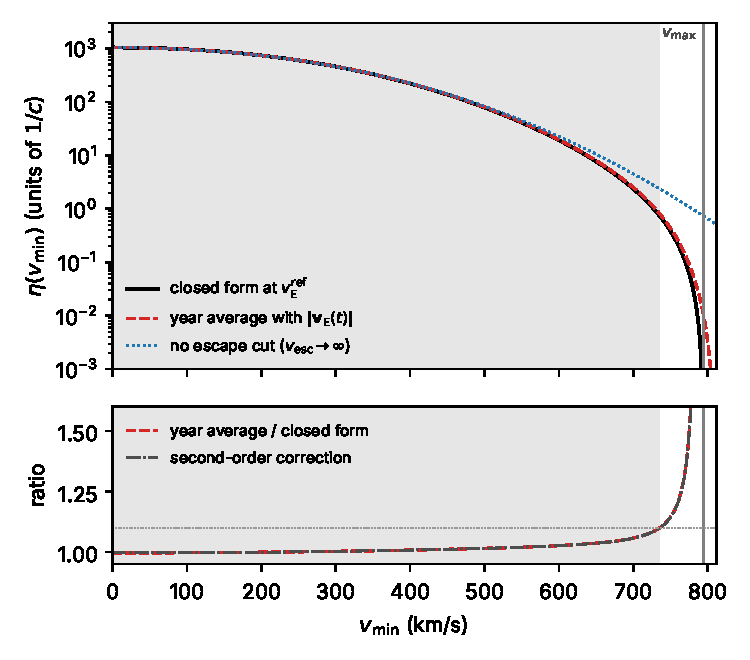
\includegraphics[width=\linewidth]{figures/ch21/limit21_1a.pdf}
\captionof{figure}{Mean inverse speed of the standard halo ($v_0 = \SI{238}{km.s^{-1}}$, $v_{\mathrm{esc}} = \SI{544}{km.s^{-1}}$) against $\vmin$. Top, in units of $1/c$: the closed form at the reference Earth speed $v_{\mathrm{E}}^{\mathrm{ref}} = \SI{250.5}{km.s^{-1}}$ (solid). Dashed: the fuller result, the same closed form averaged over a year with the exact Earth speed of \cref{eq:1.2-vE,eq:1.2-vorb} on 7305 equally spaced days. Dotted: the Maxwellian without the escape cut at $v_{\mathrm{E}}^{\mathrm{ref}}$. Bottom: the yearly average over the closed form (dashed) and the second-order correction \cref{eq:21.1-annualcorr} (dash-dotted). Gray: $\vmin \le \SI{735.6}{km.s^{-1}}$, where the yearly average exceeds the closed form at $v_{\mathrm{E}}^{\mathrm{ref}}$ by less than 10 percent (1 percent up to \SI{430.3}{km.s^{-1}}). The second-order correction stays within 1 percent of the yearly average up to \SI{786.3}{km.s^{-1}}. Vertical line: $v_{\mathrm{max}} = \SI{794.5}{km.s^{-1}}$.}\label{fig:21-limit-eta}
\par}
\smallskip
Within \SI{59}{km.s^{-1}} of $v_{\mathrm{max}}$ the yearly average exceeds the fixed-speed form by more than 10 percent, and above $v_{\mathrm{max}}$ it vanishes while the average stays positive up to \SI{810.4}{km.s^{-1}}.
\end{limitbox}
\noindent At $\vmin = 0$ the yearly average is 0.9965 of the closed form: the mean inverse speed itself barely moves. The ratio grows to 1.015 at \SI{500}{km.s^{-1}}, 1.026 at 600 and 1.057 at \SI{700}{km.s^{-1}}, then turns up steeply, to 1.20 at 760 and 1.78 at \SI{780}{km.s^{-1}}. The second-order term follows it within a few parts in a thousand to \SI{780}{km.s^{-1}}. The escape cut matters over a much wider range than the annual average does: without it, $\eta$ would be 1.18 times larger at \SI{600}{km.s^{-1}}, 1.90 times at 700 and 6.8 times at \SI{760}{km.s^{-1}}. Averaging $\eta$ over the year raises this silicon rate by 0.9 percent at \SI{10}{MeV} and by 5.6 percent at \SI{1}{MeV}, where the kernel opens near \SI{460}{km.s^{-1}}. Closer to the threshold mass the correction grows without bound, and \cref{sec:21.3} treats that regime.

\Cref{fig:21-kernel} shows the kernel of the silicon electron-recoil channel for a heavy mediator, built from the random-phase loss function with local fields of the tables of \cref{sec:10.2}, counted from their gap of \SI{1.17}{eV}. At \SI{10}{MeV} it opens at $v_{\mathrm{on}} = \SI{145}{km.s^{-1}}$, which is $(2\omega/\mchi)^{1/2}$ at the gap; the kernel, scaled to a rate per target mass as in \cref{fig:21-kernel}, is $\num{1.77e4}$ per kilogram and year at \SI{300}{km.s^{-1}}, $\num{1.28e5}$ at \SI{500}{km.s^{-1}} and $\num{3.11e5}$ at $v_{\mathrm{max}}$, for $\sigmae = \SI{e-37}{cm^2}$. Integrated against $F_\chi$ at $v_{\mathrm{E}}^{\mathrm{ref}}$, it returns \SI{5.897e4}{kg^{-1}.yr^{-1}}, the rate of \cref{sec:10.2-corrections}, and the form \cref{eq:21.1-etaform} returns the same number to five digits. At \SI{1}{MeV} the kernel opens only near \SI{460}{km.s^{-1}} and the rate, \SI{16.5}{kg^{-1}.yr^{-1}}, comes entirely from the fastest fifth of the halo. At \SI{100}{MeV} it opens at \SI{46}{km.s^{-1}} and changes by a factor of 4.0 between 300 and \SI{700}{km.s^{-1}}, against 14 at \SI{10}{MeV}. The heavier the particle, the flatter the kernel over the bulk of the halo, and the less the rate depends on the shape of $F_\chi$.
\begin{figure}[tbp]
  \centering
  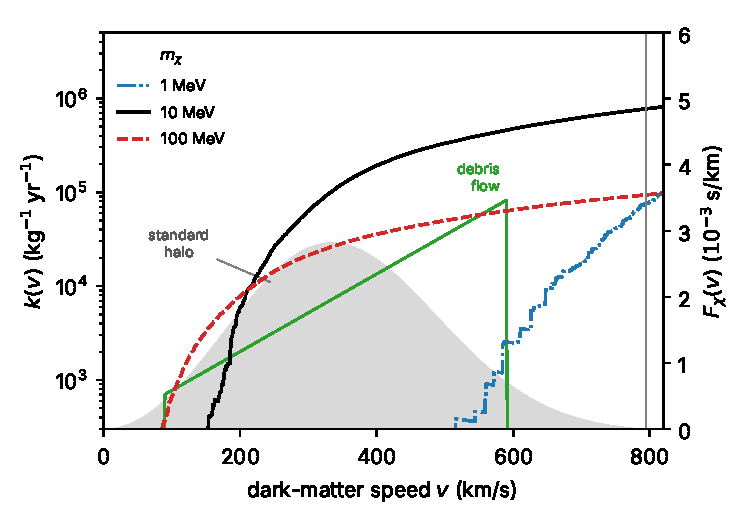
\includegraphics[width=0.8\linewidth]{figures/ch21/fig21_1.pdf}
  \caption{Rate kernel of the silicon electron-recoil channel, $\rho_\chi\varGamma(v)/\mchi\rho_T$ of \cref{eq:21.1-gammav}, the rate per unit target mass if all dark matter moved at speed $v$, for a heavy mediator, $\sigmae = \SI{e-37}{cm^2}$ and $\rho_\chi = \SI{0.3}{GeV.cm^{-3}}$, at $\mchi = 1$, 10 and \SI{100}{MeV} (left axis). The response is the direction-averaged random-phase loss function with local fields of Knapen, Kozaczuk and Lin~\cite{knapen2021dark} (\cref{sec:10.2}), from their gap of \SI{1.17}{eV}. Right axis: laboratory speed distributions at $v_{\mathrm{E}}^{\mathrm{ref}} = \SI{250.5}{km.s^{-1}}$ of the standard halo (gray, \cref{eq:1.2-Fspeed}) and of a debris flow of galactic speed \SI{340}{km.s^{-1}} (green, \cref{eq:21.1-fflow}). Vertical line: $v_{\mathrm{max}} = \SI{794.5}{km.s^{-1}}$.}
  \label{fig:21-kernel}
\end{figure}

\subsection{Threshold masses as floors}\label{sec:21.1-floor}

Where the kernel vanishes, so does the rate. By \cref{eq:21.1-functional}, a mass gives a nonzero rate only if the halo holds particles faster than $v_{\mathrm{on}}(\mchi)$. For a response whose onset $E_{\mathrm{th}}$ does not depend on $q$, the smallest $\vmin$ is $(2E_{\mathrm{th}}/\mchi)^{1/2}$ (\cref{sec:1.3}), and the condition $v_{\mathrm{on}} < v_{\mathrm{max}}$ is $\mchi > 2E_{\mathrm{th}}/v_{\mathrm{max}}^2$, the threshold mass of \cref{eq:1.3-mmin}. Quoted with $v_{\mathrm{max}} = v_{\mathrm{esc}} + v_{\mathrm{E}}^{\mathrm{ref}}$, that value is a floor, never the edge of a limit.

The onset of a real response depends on $q$. Then $v_{\mathrm{on}} = \min_q[E_{\mathrm{th}}(q)/q + q/2\mchi]$ lies above $(2E_{\mathrm{th}}/\mchi)^{1/2}$ with $E_{\mathrm{th}}$ the global minimum, and the edge lies above the floor. In silicon the floor at the gap, \SI{1.170}{eV}, is \SI{0.3332}{MeV}, and at the lowest excitation, the $1s$ exciton at \SI{1.1553}{eV}, it is \SI{0.3290}{MeV}; the edges of the pair channels lie above it (\cref{tab:9-edges}).

Near $v_{\mathrm{max}}$ the mean inverse speed $\eta$ vanishes quadratically (\cref{eq:1.3-edge}), and the reachable part of the response shrinks with it. A finite exposure therefore excludes only masses some distance above the floor, and how far above depends on the exposure, on the onset exponent of the response and on the tail of the halo. \Cref{sec:21.3} derives that distance.

The floor depends on the halo and on the Earth speed it is computed with. The reference speed fixes $v_{\mathrm{max}} = \SI{794.5}{km.s^{-1}}$ by convention (\cref{app:A.8}). In June the fastest particles move at $v_{\mathrm{esc}} + |\vect{v}_{\mathrm{E}}| = \SI{810.4}{km.s^{-1}}$, and an exposure that includes June has a nonzero rate down to a floor 3.9 percent lower, \SI{0.3202}{MeV} for the silicon gap; \cref{lim:21.1a} shows its origin in $\eta$. The annual motion is known kinematics, not an uncertainty: a limit uses the rate averaged over its exposure, June included (\cref{sec:21.3-degeneracy}), and the floor at the reference speed is the convention for comparing targets. Conversely, a halo component lowers the floor only if it carries particles faster than $v_{\mathrm{max}}$. A debris flow at \SI{340}{km.s^{-1}} reaches at most \SI{590.5}{km.s^{-1}} in the laboratory, and on its own it would give no silicon electron recoil below \SI{0.6031}{MeV}.

\subsection{A halo with a debris flow}\label{sec:21.1-debris}

Kuhlen, Lisanti and Spergel model the debris flow as an isotropic shell in velocity space: every particle has the same galactic speed $v_{\mathrm{flow}}$, in a random direction~\cite{kuhlen2012direct}. In the laboratory a particle of direction $\hat{\vect{v}}_{\mathrm{gal}}$ has speed $v$ with $v^2 = v_{\mathrm{flow}}^2 + v_{\mathrm{E}}^2 - 2v_{\mathrm{flow}}v_{\mathrm{E}}\cos\theta_{\mathrm{flow}}$, where $\theta_{\mathrm{flow}}$ is the angle between $\vect{v}_{\mathrm{gal}}$ and $\vect{v}_{\mathrm{E}}$. Since $\cos\theta_{\mathrm{flow}}$ is uniform on $[-1,1]$ and $v\,\dd v = -v_{\mathrm{flow}}v_{\mathrm{E}}\,\dd\cos\theta_{\mathrm{flow}}$, the laboratory speed distribution is~\cite[Eq.~(7)]{kuhlen2012direct}
\begin{equation}
  F_{\mathrm{flow}}(v) = \frac{v}{2v_{\mathrm{flow}}v_{\mathrm{E}}}\quad\text{for } |v - v_{\mathrm{flow}}| < v_{\mathrm{E}} ,
  \label{eq:21.1-fflow}
\end{equation}
and zero outside, for $v_{\mathrm{flow}} > v_{\mathrm{E}}$. Its mean inverse speed is $\eta_{\mathrm{flow}}(u) = 1/v_{\mathrm{flow}}$ for $u < v_{\mathrm{flow}} - v_{\mathrm{E}}$, falls linearly as $(v_{\mathrm{flow}} + v_{\mathrm{E}} - u)/(2v_{\mathrm{flow}}v_{\mathrm{E}})$ across the window, and vanishes above $v_{\mathrm{flow}} + v_{\mathrm{E}}$~\cite[Eq.~(8)]{kuhlen2012direct}. The halo is $f_\chi = (1 - p_{\mathrm{flow}})f_{\mathrm{SHM}} + p_{\mathrm{flow}}f_{\mathrm{flow}}$ at fixed total density, and in Via Lactea~II $p_{\mathrm{flow}} = 0.22$ and $v_{\mathrm{flow}} = \SI{340}{km.s^{-1}}$~\cite[Eq.~(10) and Fig.~6]{kuhlen2012direct}. Compared to the standard halo at the reference Earth speed, the flow has fewer slow particles, $\langle1/v\rangle = 1/v_{\mathrm{flow}}$, or 882 in natural units against 1041, and more fast ones: 55 percent of its particles move faster than \SI{400}{km.s^{-1}}, against 36 percent. It has none above \SI{590.5}{km.s^{-1}}.

\begin{workedexample}{The silicon rate in a halo with a debris flow}\label{we:21-debris}
Take silicon, $\mchi = \SI{10}{MeV}$, a heavy mediator and $\sigmae = \SI{e-37}{cm^2}$, with the kernel of \cref{fig:21-kernel} and $v_{\mathrm{E}} = v_{\mathrm{E}}^{\mathrm{ref}}$ for both components. The flow occupies $89.5 < v < \SI{590.5}{km.s^{-1}}$. Inserting \cref{eq:21.1-fflow} in \cref{eq:21.1-functional}, the factor $v$ of $F_{\mathrm{flow}}$ meets the factor $1/v$ of the kernel:
\begin{equation*}
  \mathcal{R}_{\mathrm{flow}} = \frac{1}{2v_{\mathrm{flow}}v_{\mathrm{E}}}\int_{v_{\mathrm{flow}} - v_{\mathrm{E}}}^{v_{\mathrm{flow}} + v_{\mathrm{E}}}\dd v\;v\,\frac{\rho_\chi\varGamma(v)}{\mchi\rho_T}
  = \frac{1}{v_{\mathrm{flow}}}\Bigl\langle v\,\frac{\rho_\chi\varGamma(v)}{\mchi\rho_T}\Bigr\rangle_{\mathrm{window}} .
\end{equation*}
Across the window the kernel rises from zero below \SI{145}{km.s^{-1}} through \SI{1.77e4}{kg^{-1}.yr^{-1}} at \SI{300}{km.s^{-1}}, \num{6.97e4} at 400 and \num{1.28e5} at \SI{500}{km.s^{-1}}, to \SI{1.82e5}{kg^{-1}.yr^{-1}} at \SI{590}{km.s^{-1}}. The mean of $v$ times the kernel over the window is \SI{2.769e7}{km.s^{-1}.kg^{-1}.yr^{-1}}, and
\begin{equation*}
  \mathcal{R}_{\mathrm{flow}} = \frac{\SI{2.769e7}{km.s^{-1}.kg^{-1}.yr^{-1}}}{\SI{340}{km.s^{-1}}} = \SI{8.145e4}{kg^{-1}.yr^{-1}} ,
\end{equation*}
the rate if all of the dark matter were in the flow. The form \cref{eq:21.1-etaform} with $\eta_{\mathrm{flow}}$ gives the same number. Per particle the flow is 1.381 times as effective as the standard halo, $\mathcal{R}_{\mathrm{SHM}} = \SI{5.897e4}{kg^{-1}.yr^{-1}}$, because it puts more particles where the kernel is large.

The mixed halo, by linearity, gives
\begin{equation*}
  \mathcal{R} = 0.78\times\num{5.897e4} + 0.22\times\num{8.145e4} = \SI{6.392e4}{kg^{-1}.yr^{-1}} ,
\end{equation*}
8.4 percent above the standard halo, or 175 events per kilogram and day. The spectrum hardly changes shape: its mean moves from 6.59 to \SI{6.62}{eV}. The flow's own spectrum ends at \SI{19.4}{eV}, the largest energy a particle at \SI{590.5}{km.s^{-1}} can deposit, against \SI{35}{eV} for the standard halo, and it peaks near \SI{6.0}{eV}, against \SI{5.4}{eV}.

The same halo changes the rate differently at other masses. For a light mediator at \SI{10}{MeV} the mixed rate is 8.8 percent above the standard one, and for a heavy mediator at \SI{100}{MeV}, 5.2 percent. At \SI{1}{MeV}, where the kernel opens near \SI{460}{km.s^{-1}}, the flow is only 0.28 times as effective as the standard halo, and the mixed rate falls 16 percent below it. A debris flow moves particles from both tails of the speed distribution into its middle. It raises the rate where the kernel opens in the bulk of the halo and lowers it near the threshold mass, which stays at the floor set by the standard component.
\end{workedexample}
